% MathMode: full, MathRender: svg, MathDpi: 300, MathEmbedLimit: 524288, MathScale: 105, MathBaseline: 0, MathDocClass: [10pt]book, MathImgDir: math, MathLatex: latex, MathSvgFontFormat: "", MathSvgSharePaths: True, MathSvgPrecision: 3, Dvisvg: dvisvgm
\documentclass[10pt]{book}
% generated by Madoko, version 1.1.4
%mdk-data-line={1}
\newcommand\mdmathmode{full}
\newcommand\mdmathrender{svg}
\usepackage[heading-base={2},section-num={false},bib-label={true},fontspec={true}]{madoko2}
\usepackage{tikz}
\usepackage{tikz-cd}


\begin{document}


\begin{mdSnippets}
%mdk-data-line={8;./src/article/../mytheme/myprelude.mdk:103}
%mdk-data-line={8;./src/article/../mytheme/myprelude.mdk:129}
%mdk-begin-mathdefs
%mdk-data-line={8;./src/article/../mytheme/myprelude.mdk:138}
\newcommand{\downsetlattice}[1]{\mathcal{O}(#1)}
\newcommand{\downX}[1]{\downarrow #1}
\newcommand{\powerset}[1]{\mathbb{P}(#1)}
\newcommand{\dual}[1]{{#1^{\mathrm{op}}}}
\newcommand{\defset}[2]{\{#1 \mid #2\}}
\newcommand{\maxel}{\mathrm{Max}}
\newcommand{\minel}{\mathrm{Min}}

%mdk-data-line={131}
\begin{mdDisplaySnippet}[82aea3235194d22c2009e897a35179c8]%mdk
%mdk-data-line={138}
 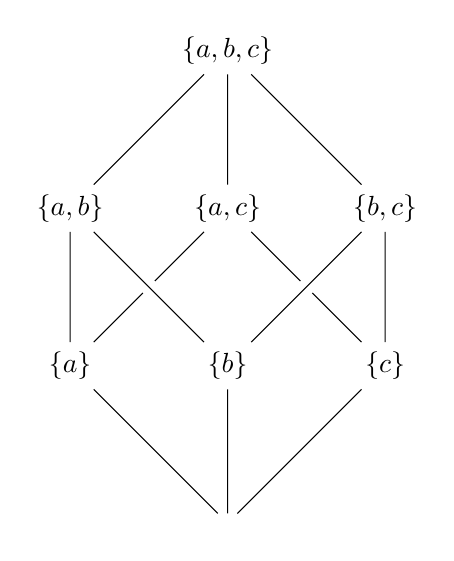
\begin{tikzpicture}
\node (max) at (0,4) {$\{a, b, c\}$};
\node (a) at (-2,2) {$\{a, b\}$};
\node (b) at (0,2) {$\{a, c\}$};
\node (c) at (2,2) {$\{b, c\}$};
\node (d) at (-2,0) {$\{a\}$};
\node (e) at (0,0) {$\{b\}$};
\node (f) at (2,0) {$\{c\}$};
\node (min) at (0,-2) {$\varnothing$};
\draw (min) -- (d) -- (a) -- (max) -- (b) -- (f)
(e) -- (min) -- (f) -- (c) -- (max)
(d) -- (b);
\draw[preaction={draw=white, -,line width=6pt}] (a) -- (e) -- (c);
\end{tikzpicture}\end{mdDisplaySnippet}%mdk
%mdk-data-line={178}

\end{mdSnippets}

\end{document}
